\clearpage
\title{Problem 4.2}
\author{}
\date{}
\maketitle

\section*{Problem Description}
Write a code to take input from user as Hexadecimal and output it as Hexadecimal.

\section*{Process}
\subsection*{Code:}

\begin{multicols}{2}{|}
    \begin{minted}[linenos,breaklines,breakanywhere]{nasm}
DATA SEGMENT
    CR EQU 0DH
    LF EQU 0AH
    CNT DB 4
DATA ENDS

CODE SEGMENT 
    ASSUME CS: CODE, DS: DATA
    
START:
    MOV AX, DATA
    MOV DS, AX
    
    XOR BX, BX
    MOV CX, 4
    
    MOV AH, 1
    INT 21H
    
INPUT:
    CMP AL, 0DH
    JE EXIT
    
    CMP AL, 39H
    JG LETTER
    
    AND AL, 0FH
    JMP SHIFT
    
LETTER:
    SUB AL, 37H    
    
SHIFT:
    SHL BX, CL
    OR BL, AL
    
    INT 21H
    
    JMP INPUT    

EXIT: 
    MOV DL, CR
    MOV AH, 2
    INT 21H
    MOV DL, LF
    INT 21H
    
PRINT:    
    MOV DL, BH
    SHR DL, 4
    ROL BX, 4
    
    CMP DL, 10 
    JL CONV_NUM
    JGE CONV_CHAR
    
CONV_NUM:
    OR DL, 30H
    MOV AH, 2
    INT 21H
    
    LOOP PRINT
    
CONV_CHAR:
    SUB DL, 9
    OR DL, 40H
    MOV AH, 2
    INT 21H

    LOOP PRINT

END1:
    MOV AH, 4CH
    INT 21H
    
CODE ENDS
ENDS START   
\end{minted}
\end{multicols}

\subsection*{Output}
\begin{center}
    \centering
    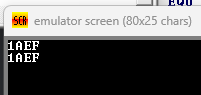
\includegraphics[width = .4\textwidth]{HEX.png}
    \captionof{figure}{Hexadecimal input \& output}
\end{center}


